\documentclass[conference]{IEEEtran}
\IEEEoverridecommandlockouts
% The preceding line is only needed to identify funding in the first footnote. If that is unneeded, please comment it out.
\usepackage{cite}
\usepackage{amsmath,amssymb,amsfonts}
\usepackage{algorithm}  
\usepackage{algpseudocode}
\usepackage{graphicx}
\usepackage{textcomp}
\usepackage{xcolor}
\def\BibTeX{{\rm B\kern-.05em{\sc i\kern-.025em b}\kern-.08em
    T\kern-.1667em\lower.7ex\hbox{E}\kern-.125emX}}
\begin{document}

\title{
    Finite Element Method for 2D Heat Equation
}

\author{
\IEEEauthorblockN{1\textsuperscript{st} Tianyuan Wu}
\IEEEauthorblockA{\textit{ShanghaiTech University} \\}
\and
\IEEEauthorblockN{2\textsuperscript{nd} Mengying Wu}
\IEEEauthorblockA{\textit{ShanghaiTech University} \\}
}

\maketitle

\begin{abstract}
In this paper, we implement a fast, parallel finite element method solver for 2D heat 
equation, a mesh generator based on delaunay triangulation and a GUI which is able to 
show the dynamic changes of temperature ($T(x, y)$) by time ($t$) of a given region with 
initial conditions. Then, we test our solver on differentregions and different boundary 
conditions. Also, we analysis the error between our numeric solution and the anylatical solution.
\end{abstract}

\begin{IEEEkeywords}
Finite element method, Heat equation, Delaunay triangulation, Error analysis
\end{IEEEkeywords}


\section{Introduction}
Finite element method (FEM) is the most commonly used method for solving differential equations of 
engineering and mathematical models, such as structural analysis, heat transfer and fluid flow\cite{b1}.
Our work focus on the application of FEM in solving 2D heat equation, error analysis of 
FEM in special designed problems and visualization of heat transfer. It basically 
includes 3 parts: (1) The FEM solver for 2D heat equation; (2) The mesh construction algorithm; 
(3) The heat transfer visualization and animation part. All 3 parts are implemented in Python, 
with third-party libraries \texttt{numpy}\cite{b8} (for matrix computations), \texttt{scipy}\cite{b10} (for basic 
linear algebra support, like solving linear equations), and \texttt{matplotlib}\cite{b9} (for animation 
and visualization)


\section{2D Heat Equation}
Heat equation is a certain partial differential equation which describes the heat transfers in a specific system. 
The 2-dimensional form of the equation is known as:
\begin{align}\nonumber
    \frac{\partial{T}}{\partial{t}} = \lambda(\frac{\partial {^2 T}}{\partial{x^2}} + \frac{\partial {^2 T}}{\partial{y^2}}) + f(x, y, t)
\end{align}
Where $T = T(x, y, t)$ is the heat (or temperature) of given position $(x, y)$ at time point $t$, 
$f(x, y, t)$ describes the external heat given to the system, which is similar to the ``external force'' 
in mechanics and $\lambda$ is a given constant describes the property of the system.\\
To solve a specific 2D heat transfer problem, the following conditions must be specified first:
\begin{enumerate}
    \item The region $\Omega$ and the initial condition in $\Omega$:
        \begin{align}\nonumber T_{\Omega, initial} = T_{\Omega}(x, y, 0) \end{align}
    \item Neummann boundary conditions
        \begin{align}\nonumber \frac{\partial{T}}{\partial{\vec{n}}}\big |_{\partial{\Omega_n}} = T_{n} \end{align}
    \item Dirichlet boundary conditions
        \begin{align}\nonumber T\big| _{\partial{\Omega_d}} = T_{d} \end{align}
\end{enumerate}
Once the initial condition, Dirichlet and Neummann boundary conditions are specified, 
we can simulate the state of the system at any time.


\section{Methods}
    \subsection{Finite Difference Method}
    This equation is actually a 3-dimensional partial differential equation, which is computational 
    expensive if we use a pure FEM solver. Hence, we use finite difference method to discretize
    the time dimension:
    \begin{align}\nonumber
        & \frac{T(x,y, t_{n+1}) - T(x, y, t_{n})}{dt} =\\
        \nonumber& \lambda(\frac{\partial {^2 T(x, y, n+1)}}{\partial{x^2}} + \frac{\partial {^2 T(x, y, n+1)}}{\partial{y^2}}) + f(x, y, t_{n+1})
    \end{align}
    To simplify the problem, we take $\lambda = 1$, and denote $\frac{\partial {^2 T_n}}{\partial{x^2}} + \frac{\partial {^2 T_n}}{\partial{y^2}}$ 
    as $\Delta T_n$, so the equation can be written as:
    $$\frac{T_{n+1} - T_{n}}{dt} = \Delta T_{n+1} + f_{n+1}$$
    To maintain the stability of the solution, we use the implicit Euler form of this equation:
    $$T_{n+1}(1 - \Delta T_{n+1} dt) = f_{n+1}dt + T_{n}$$
    Consequently, once the heat distribution at $t = n$ is computed by FEM, we can calculate the solution at $t = n + 1$
    by finite difference method with limited error rate.

    \subsection{Finite Element Method}
    By finite difference method, the 3-dimensional problem is simplified into two dimensions, then we will apply finite 
    element method to solve it.
    Suppose we discretize the region into $k$ nodes $\{n_1, n_2,\ldots, n_k\}$, which make up $m$ triangle mesh $\{m_1, m_2,\ldots,  m_p\}$, 
    Then the discreted solution is:
    $$T_{sol} = T_{sol, d} + T_{rest}$$
    where $T_{sol, d}$ is to fit the Dirichlet boundaries.\\
    Then, we use Galerkin's method to solve $T_{rest}$. Denote $\{\phi_1, \phi_2, \ldots, \phi_k\}$ as the basis of $k$ nodes. 
    For each base function $\phi$, we have
    $$\phi_j(N_i) = \begin{cases} 1, \quad i = j\\ 0, \quad \text{otherwise}\end{cases}$$
    The visualization of this base function is shown in Fig.1.\cite{b2} 
    \newpage
    \begin{figure}[h]
        \centering
        \includegraphics[scale=0.5]{/home/wuty/Pictures/fem.png}
        \caption{Visualization of a 2D base function}
    \end{figure}
    Notice that, the following equation holds for any base function $\phi_j$:
    \begin{equation}\nonumber
        \begin{aligned}
            & \int\limits_\Omega T_{rest, n} \phi_j dx+(\int\limits_\Omega \nabla T_{rest, n} \cdot \nabla \phi_j dx) \cdot dt =\\
            & \int\limits_\Omega T_{rest, n-1}\phi_j dx+(\int\limits_{\partial\Omega_n} T_{rest, n}^{neum} \phi_jds)\cdot dt+(\int\limits_\Omega f_n \phi_j dx)\cdot dt
        \end{aligned}
    \end{equation}
    And $T_{rest}$ and time $t$ can be represented as a linear combination of all basis.
    $$T_{rest, t} = \sum_{i=1}^{k}\alpha_i\phi^{i}_{t}$$
    To convert the integral equation into a linear system which is convienent of solving by computers, we construct the mass matrix $M$:
    $$M_{ij} = \sum\limits_{A\in Tri} \int\limits_A \phi_i  \phi_j dx$$
    and the stiffness (coefficient) matrix $A$:
    $$A_{ij} = \int\limits_\Omega\nabla \phi_i \cdot \nabla \phi_j dx$$
    Finally, we can construct the following linear system:
    \begin{equation}\nonumber
        \begin{aligned}
        & (Adt+M)T_{rest,n} = MT_{rest,n-1} \\
        & +(\int\limits_{\partial\Omega_n} T_{rest, n}^{neum} \phi_jds)\cdot dt+(\int\limits_\Omega f_n \phi_j dx)\cdot dt
        \end{aligned}
    \end{equation}
    
    \subsection{Mesh Construction - Delaunay Triangulation}
    Another key difference between 1D and 2D problems is, we need a proper method to generate triangle mesh for the FEM solver.
    For this problem, we refer to the Delaunay triangulation\cite{b4}\cite{b5}\cite{b7}, which is a triangulation algorithm for a given 
    set of discrete points $P$ such that no point in $P$ is inside the circumcircle of any triangle in $DT(P)$. Delaunay triangulations 
    maximize the minimum angle of all the angles of the triangles in the triangulation\cite{b4}.\\
    There are several algorithms available for Delaunay triangulation, here we use the Bowyer-Watson's algorithm\cite{b6}. The 
    pseudo-code of this algorithm is shown in Algorithm 1.\\
    \begin{algorithm}[h]  
        \caption{Bowyer-Watson's Algorithm}  
        \textbf{Input} Points := $\{p_1, p_2,\ldots, p_n\}$
            \begin{algorithmic}[1]  
                \State Triangulation := []
                \State Add a super triangle including all points in Triangulation
                \For {each point in Points}
                    \State badTriangles := \{\}
                    \For {each triangle in Triangulation}
                        \If point is inside triangle's circumcircle
                            \State badTriangles = badTriangles $\bigcup$ triangle
                        \EndIf
                    \EndFor
                    \State Polygon := []
                    \For {each triangle in badTriangles}
                        \For {each edge in triangle}
                            \If {edge is not shared by badTriangles}
                                \State Add edge to Polygon
                            \EndIf
                        \EndFor
                    \EndFor
                    \For {each triangle in badTriangles}
                        \State Remove triangle from Triangulation
                    \EndFor
                    \For {each edge in Polygon}
                        \State NewTriangle := Triangle(edge, point)
                        \State Add NewTriangle to Triangulation
                    \EndFor
                    \For {each triangle in Triangulation}
                        \If {triangle contains a vertex in super triangle}
                            \State Remove triangle from Triangulation
                        \EndIf
                    \EndFor
                \EndFor\\
                \Return Triangulation
            \end{algorithmic}  
        \end{algorithm}
    After one iteration of triangulation, we traverse all edges, and find which ones are longer than the given threshold.
    Then we add additional points pm these edges to split them into shorter edges. Then run Delaunay triangulation recursively, 
    until edges of all triangles are smaller enough. The triangulation result of the $1^{st}$ run is shown in Fig.2, and 
    the final result is shown in Fig.3. Also, we show the triangulation result of \texttt{scipy.spatial.Delaunay}\cite{b10} in Fig.4 
    as a benchmark for comparison. It's shown that our performance is similar to the benchmark.
    \begin{figure}[h]
        \centering
        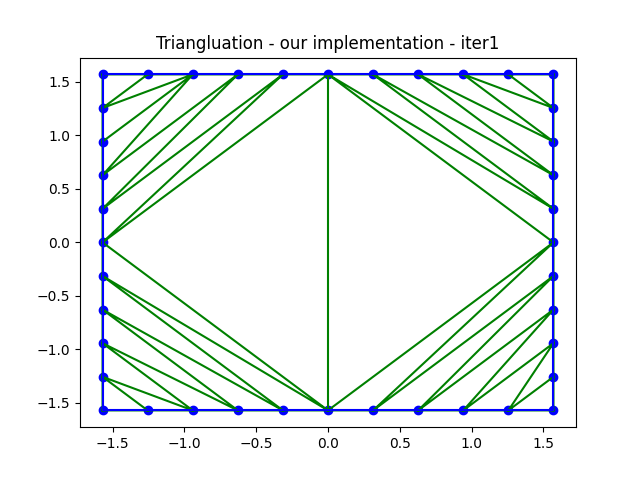
\includegraphics[scale=0.4]{../fig/tri_1st.png}
        \caption{Iteration 1 of delaunay triangulation}
    \end{figure}
    \newpage

    \begin{figure}[h]
        \centering
        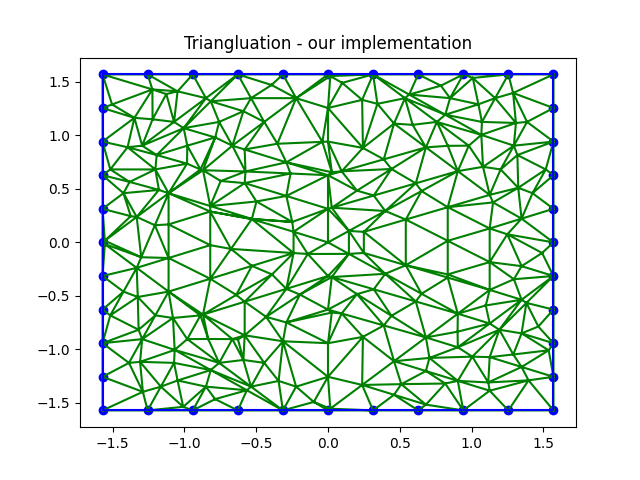
\includegraphics[scale=0.4]{../fig/tri_2nd.png}
        \caption{Triangulation result of our algorithm}
    \end{figure}

    \begin{figure}[h]
        \centering
        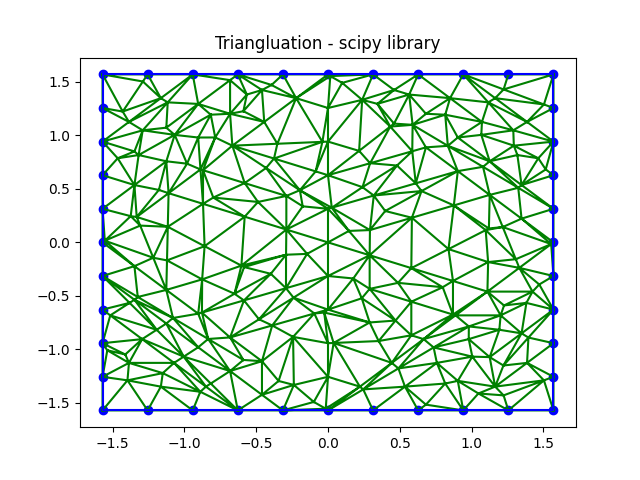
\includegraphics[scale=0.4]{../fig/tri_scipy.png}
        \caption{Benchmark (scipy)}
    \end{figure}

\section{Results}
    \subsection{Performance Evaluation}
    Our FEM solver implemented all in Python, with linear system solver \texttt{scipy.linalg.lsqr}, 
    which is fast and parallel. The test platform of our FEM solver is \texttt{Intel(R) i7-8700k} (6 core, 12 threads),
    16GB memory, with \texttt{Ubuntu 20.04}. The performance is shown in Table 1.
    \begin{table}[htbp]
        \centering
        \caption{Performance of FEM solver} 
        \begin{tabular}{|c|c|}  
            \hline
            \# of Nodes & Solving Time\\
            \hline
            253 & 3.58s\\
            \hline
            282 & 4.58s\\
            \hline
            717 & 9.42s\\
            \hline
        \end{tabular}
    \end{table}
    \subsection{Solution Visualization}
    We test our FEM solver in the region and boundary conditions shown in Fig.5. The red lines represents 
    Neummann boundary conditions, the blue lines represents the Dirichlet boundary conditions, and the green lines
    shows the triangle mesh.
    \begin{figure}[H]
        \centering
        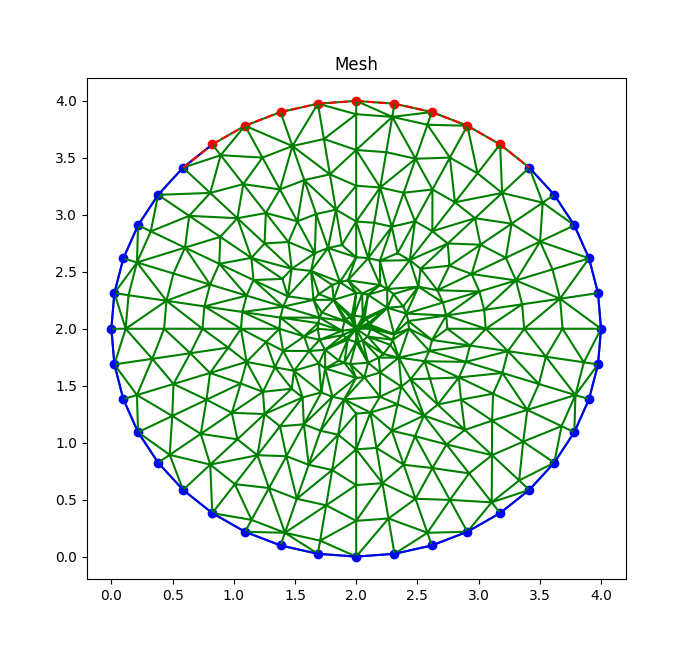
\includegraphics[scale=0.35]{../fig/mesh.png}
        \caption{Problem visualization}
    \end{figure}
    The configuration of first case is, set $f(x, y, t) = 10$, Neummann boundary $\frac{\partial{T}}{\partial{\vec{n}}}\big |_{\partial{\Omega_n}} = 0$, 
    Dirichlet boundary $T\big| _{\partial{\Omega_d}} = 0$ and the initial condition $T_{initial} = 0$. Run 100 time steps, 
    with each step 0.01s. The result is shown in Fig.6
    \begin{figure}[H]
        \centering
        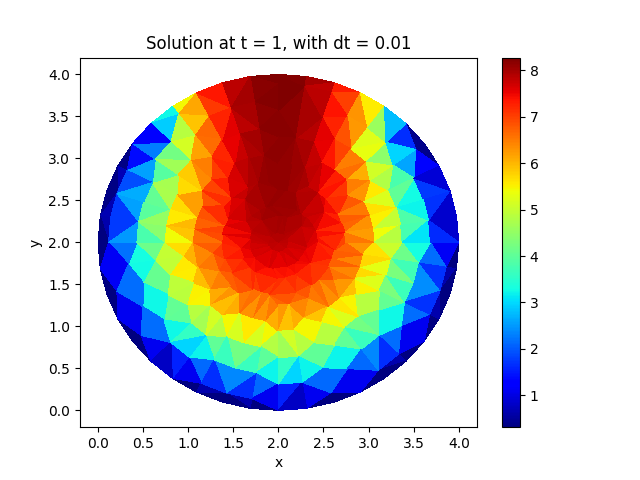
\includegraphics[scale=0.4]{../fig/ext_heat10_zero_others.png}
        \caption{Solution of case 1}
    \end{figure}
    The other conditions of the second case is the same as the first one, except the Neummann boundary 
    $\frac{\partial{T}}{\partial{\vec{n}}}\big |_{\partial{\Omega_n}} = -10$. The result is shown in Fig.7
    \begin{figure}[H]
        \centering
        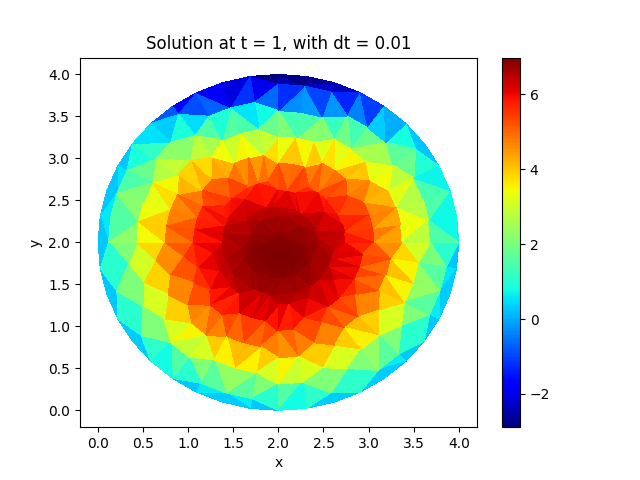
\includegraphics[scale=0.4]{../fig/ext_10_neum_-10.png}
        \caption{Solution of case 2}
    \end{figure}
    The thrid case is, set all other conditions to 0, except the Neummann boundary $\frac{\partial{T}}{\partial{\vec{n}}}\big |_{\partial{\Omega_n}} = 10$,
    and the result is shown in Fig.8
    \begin{figure}[H]
        \centering
        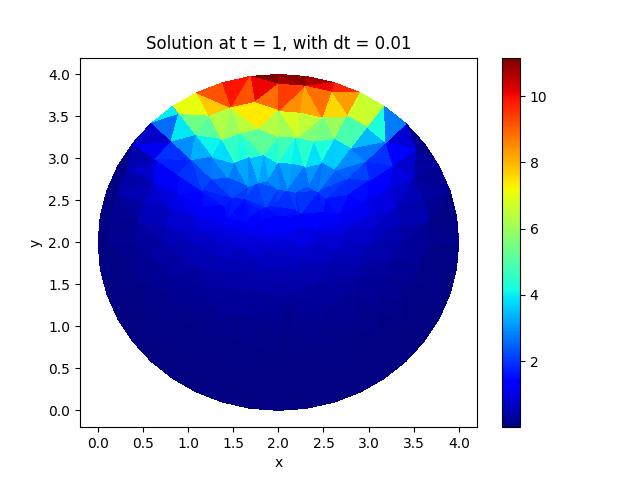
\includegraphics[scale=0.4]{../fig/no_ext_neum_10.png}
        \caption{Solution of case 2}
    \end{figure}
    Limited to the PDF format, the dynamic visualization cannot be shown in this paper. But the animation can be 
    done with \texttt{FEM\_Solver.show\_animate} in our implementation.

\section{Error Analysis}
    \subsection{Problem Construction}
    To test the accuracy of our solver, we specially designed a problem with prior anylatical solution. The problem is 
    shown in Fig.3, which is defined in $[-\frac{\pi}{2} , \frac{\pi}{2}] \times [-\frac{\pi}{2} , \frac{\pi}{2}]$, with 
    all boundary are Dirichlet boundary, and $T\big| _{\partial{\Omega_d}} = 0$. The initial state is
    $$T(x, y, 0) = cos(x)cos(y)$$
    and we can get the anylatical solution is:
    $$T(x, y, t) = cos(x)cos(y)e^{-2t}$$

    \subsection{Comparison \& Analysis}
    We simulate the following problem 100 steps with $dt = 0.01$, and the solution of our solver is shown in Fig.9, 
    while the anylatical solution is shown in Fig.10. It's no significant difference between the 2 solutions.
    \begin{figure}[H]
        \centering
        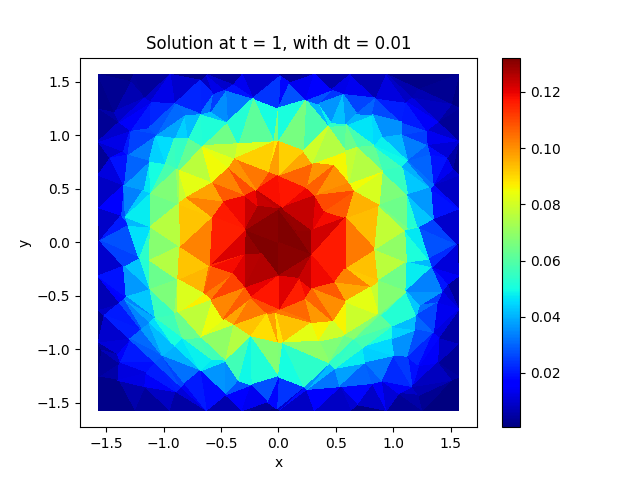
\includegraphics[scale=0.4]{../fig/sp_sol.png}
        \caption{Our solution}
    \end{figure}

    \begin{figure}[H]
        \centering
        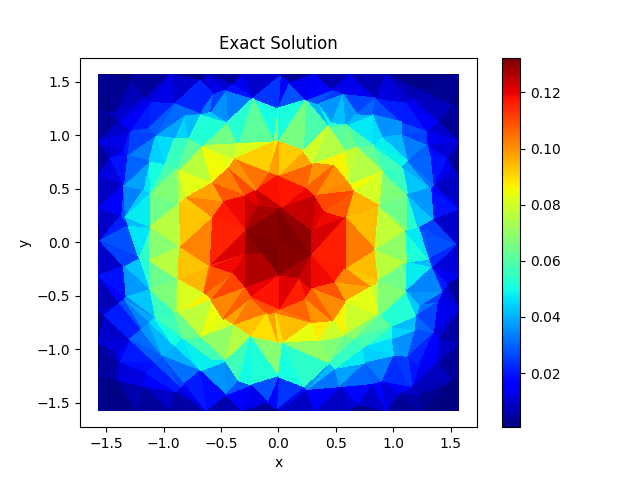
\includegraphics[scale=0.4]{../fig/sp_exact.png}
        \caption{Anylatical solution}
    \end{figure}

    Then, we analysis the error rate between the two solutions by time, and plot the error rate in Fig.11.
    We can see that the error rate is less than $1\%$, and grows linearly by time.
    \begin{figure}[H]
        \centering
        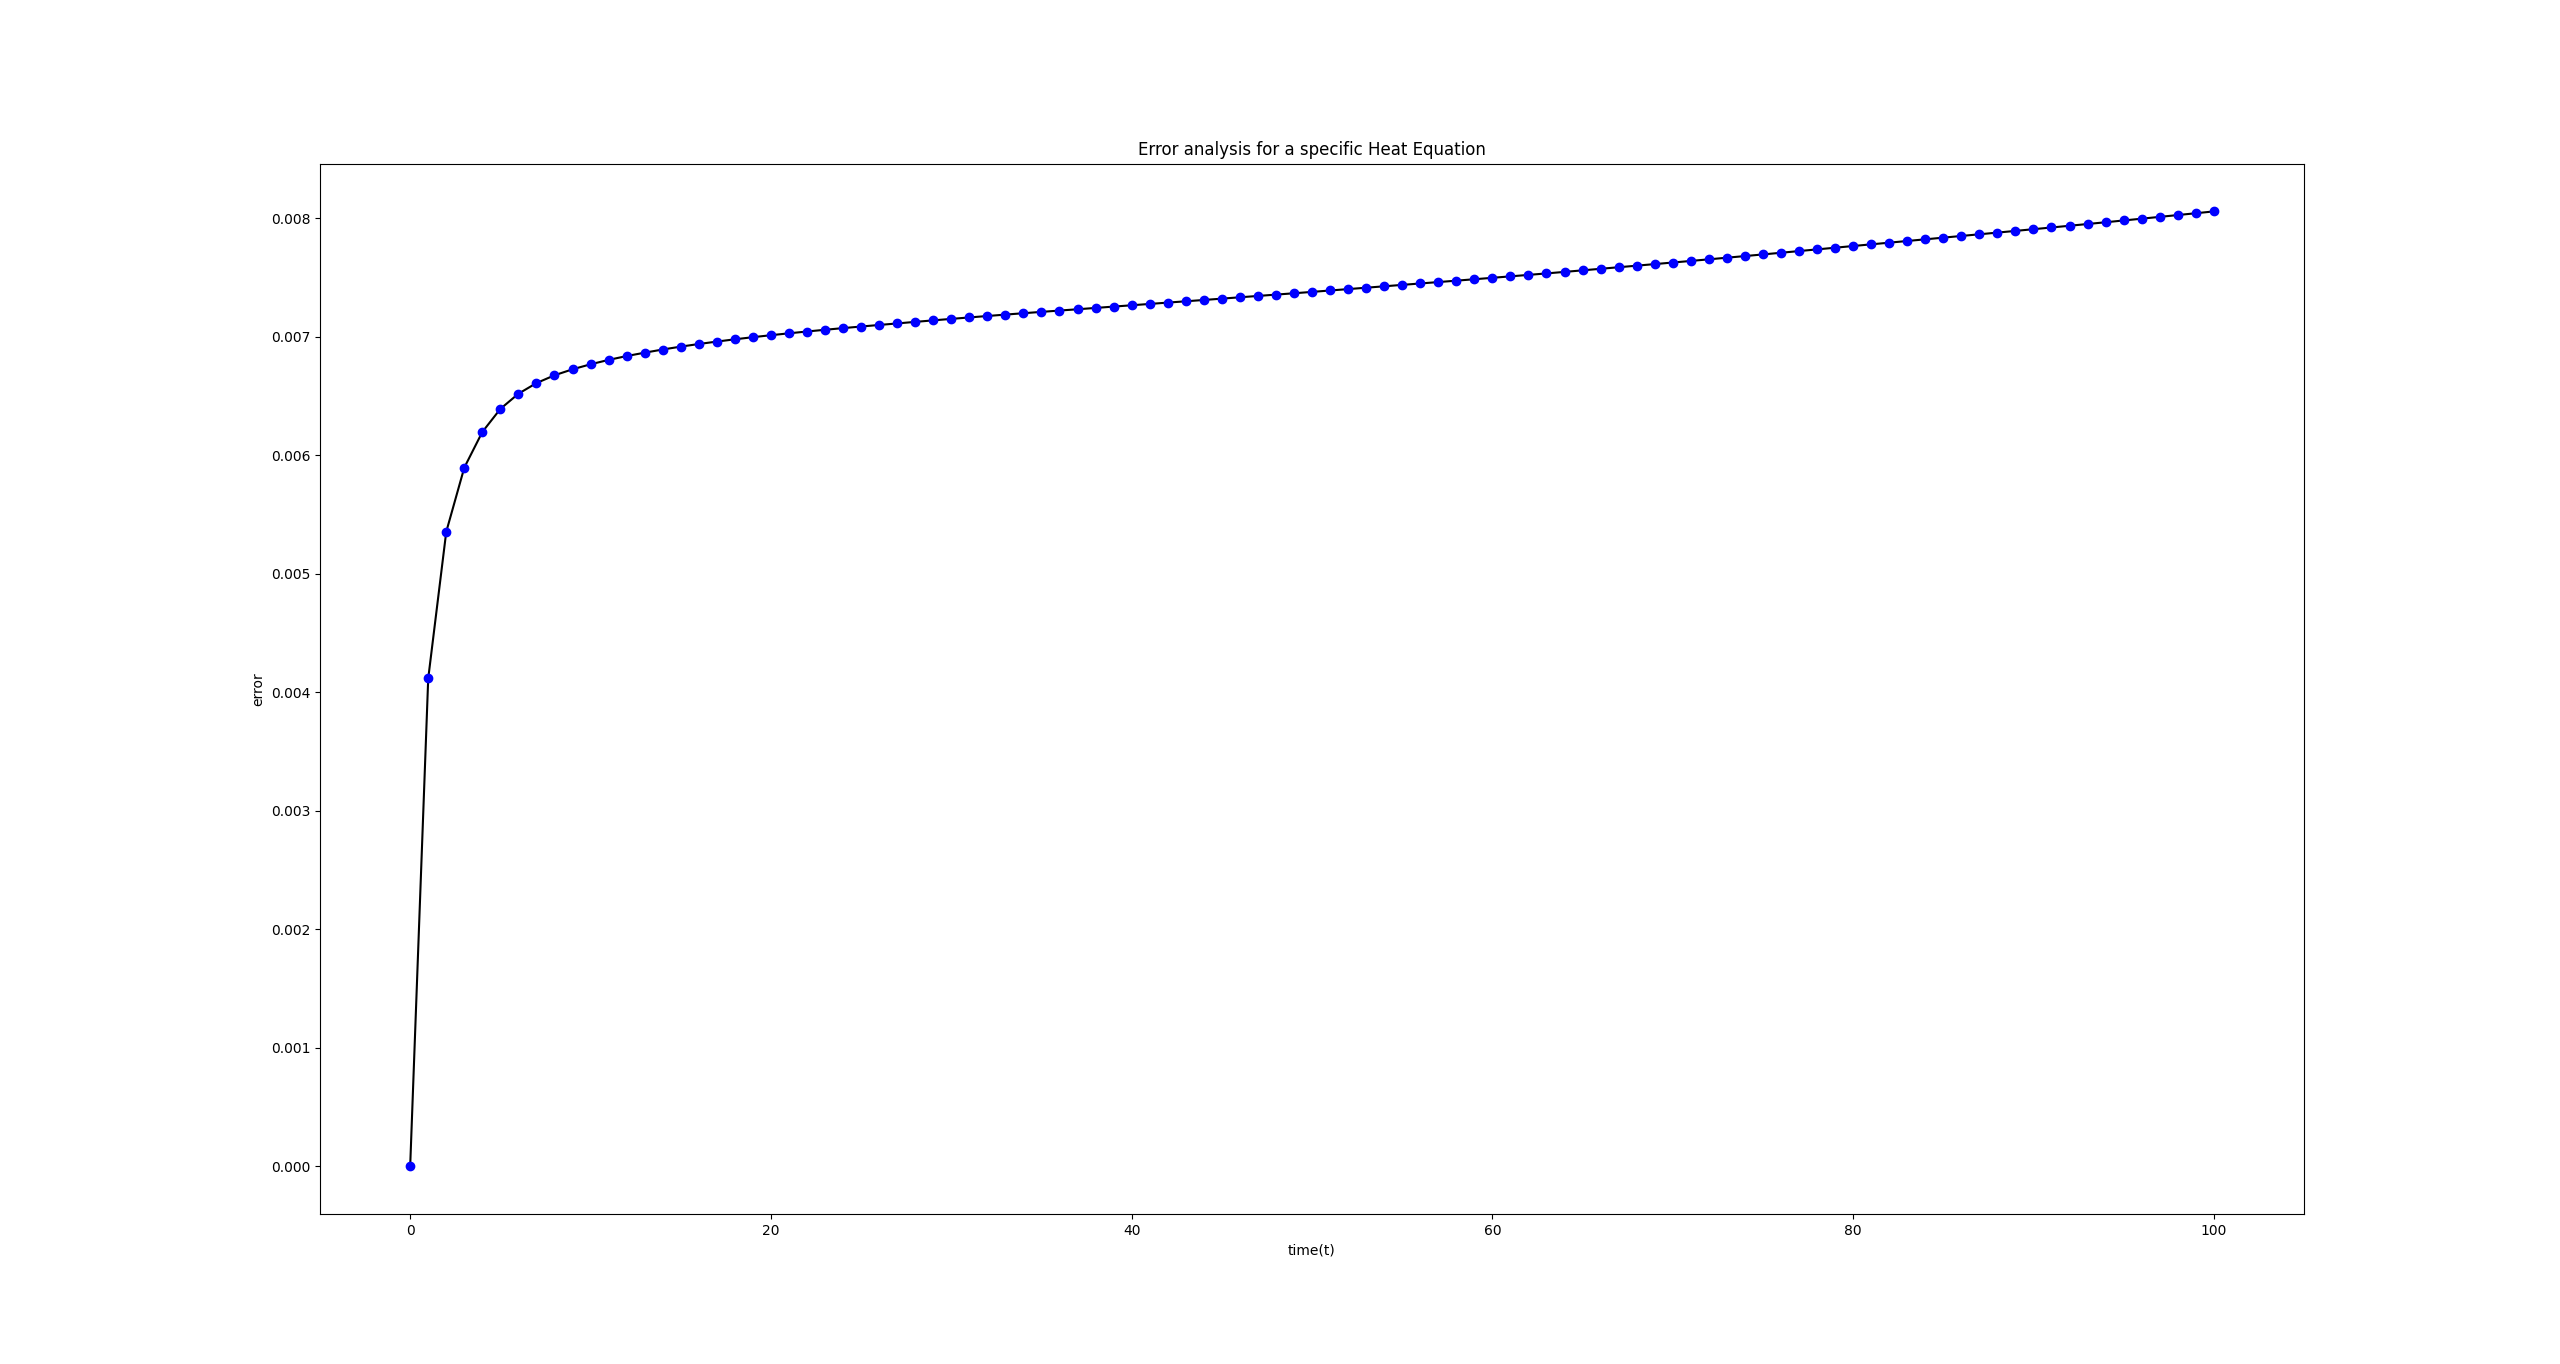
\includegraphics[scale=0.4]{../fig/err.png}
        \caption{Relationship between error and time }
    \end{figure}

\section{Conclusion}
In this work, we implement a FEM solver for 2D heat equation, and test its performance and accuracy in 
different conditions. Also, we implemented a mesh generation algorithm to construct proper mesh for 
our solver. Then, we use \texttt{matplotlib}\cite{b9} to visualize the solution, and creates animation to show 
the heat transfer. Finally, we analysis the error rate of our solver. In conclusion, our implementation 
is fast, easy for visualization and have a relative good accuracy.

\newpage
\begin{thebibliography}{00}
\bibitem{b1} Finite Element Method, wikipedia (http://en.wikipedia.org/wiki/\\Finite\_element\_method)
\bibitem{b2} M. G. Larson and F. Bengzon, The Finite Element Method: Theory, Implementation, and Applications, vol. 10. Berlin, Heidelberg: Springer Berlin Heidelberg, 2010.
\bibitem{b3} P. Ciarlet, The Finite Element Method for Elliptic Problems, NorthHolland, New York, 1980.
\bibitem{b4} Delaunay triangulation, wikipedia (http://en.wikipedia.org/wiki/\\Delaunay\_triangulation)
\bibitem{b5} M. de Berg, M. van Kreveld, M. Overmars, and O. Cheong, Computational Geometry: Algorithms and Applications. Springer-Verlag, 2008.
\bibitem{b6} Bowyer-Watson's algorithm, wikipedia (http://en.wikipedia.org/wiki/\\Bowyer\%E2\%80\%93Watson\_algorithm)
\bibitem{b7} B. Delaunay: Sur la sphere vide, Izvestia Akademii Nauk SSSR, Otdelenie Matematicheskikh i Estestvennykh Nauk, 7:793-800, 1934
\bibitem{b8} Numpy, https://numpy.org/
\bibitem{b9} Matplotlib, https://matplotlib.org/
\bibitem{b10} Scipy, https://www.scipy.org/
\end{thebibliography}
\end{document}
